% Options for packages loaded elsewhere
\PassOptionsToPackage{unicode}{hyperref}
\PassOptionsToPackage{hyphens}{url}
%
\documentclass[
]{article}
\usepackage{amsmath,amssymb}
\usepackage{iftex}
\ifPDFTeX
  \usepackage[T1]{fontenc}
  \usepackage[utf8]{inputenc}
  \usepackage{textcomp} % provide euro and other symbols
\else % if luatex or xetex
  \usepackage{unicode-math} % this also loads fontspec
  \defaultfontfeatures{Scale=MatchLowercase}
  \defaultfontfeatures[\rmfamily]{Ligatures=TeX,Scale=1}
\fi
\usepackage{lmodern}
\ifPDFTeX\else
  % xetex/luatex font selection
\fi
% Use upquote if available, for straight quotes in verbatim environments
\IfFileExists{upquote.sty}{\usepackage{upquote}}{}
\IfFileExists{microtype.sty}{% use microtype if available
  \usepackage[]{microtype}
  \UseMicrotypeSet[protrusion]{basicmath} % disable protrusion for tt fonts
}{}
\makeatletter
\@ifundefined{KOMAClassName}{% if non-KOMA class
  \IfFileExists{parskip.sty}{%
    \usepackage{parskip}
  }{% else
    \setlength{\parindent}{0pt}
    \setlength{\parskip}{6pt plus 2pt minus 1pt}}
}{% if KOMA class
  \KOMAoptions{parskip=half}}
\makeatother
\usepackage{xcolor}
\usepackage[margin=1in]{geometry}
\usepackage{color}
\usepackage{fancyvrb}
\newcommand{\VerbBar}{|}
\newcommand{\VERB}{\Verb[commandchars=\\\{\}]}
\DefineVerbatimEnvironment{Highlighting}{Verbatim}{commandchars=\\\{\}}
% Add ',fontsize=\small' for more characters per line
\usepackage{framed}
\definecolor{shadecolor}{RGB}{248,248,248}
\newenvironment{Shaded}{\begin{snugshade}}{\end{snugshade}}
\newcommand{\AlertTok}[1]{\textcolor[rgb]{0.94,0.16,0.16}{#1}}
\newcommand{\AnnotationTok}[1]{\textcolor[rgb]{0.56,0.35,0.01}{\textbf{\textit{#1}}}}
\newcommand{\AttributeTok}[1]{\textcolor[rgb]{0.13,0.29,0.53}{#1}}
\newcommand{\BaseNTok}[1]{\textcolor[rgb]{0.00,0.00,0.81}{#1}}
\newcommand{\BuiltInTok}[1]{#1}
\newcommand{\CharTok}[1]{\textcolor[rgb]{0.31,0.60,0.02}{#1}}
\newcommand{\CommentTok}[1]{\textcolor[rgb]{0.56,0.35,0.01}{\textit{#1}}}
\newcommand{\CommentVarTok}[1]{\textcolor[rgb]{0.56,0.35,0.01}{\textbf{\textit{#1}}}}
\newcommand{\ConstantTok}[1]{\textcolor[rgb]{0.56,0.35,0.01}{#1}}
\newcommand{\ControlFlowTok}[1]{\textcolor[rgb]{0.13,0.29,0.53}{\textbf{#1}}}
\newcommand{\DataTypeTok}[1]{\textcolor[rgb]{0.13,0.29,0.53}{#1}}
\newcommand{\DecValTok}[1]{\textcolor[rgb]{0.00,0.00,0.81}{#1}}
\newcommand{\DocumentationTok}[1]{\textcolor[rgb]{0.56,0.35,0.01}{\textbf{\textit{#1}}}}
\newcommand{\ErrorTok}[1]{\textcolor[rgb]{0.64,0.00,0.00}{\textbf{#1}}}
\newcommand{\ExtensionTok}[1]{#1}
\newcommand{\FloatTok}[1]{\textcolor[rgb]{0.00,0.00,0.81}{#1}}
\newcommand{\FunctionTok}[1]{\textcolor[rgb]{0.13,0.29,0.53}{\textbf{#1}}}
\newcommand{\ImportTok}[1]{#1}
\newcommand{\InformationTok}[1]{\textcolor[rgb]{0.56,0.35,0.01}{\textbf{\textit{#1}}}}
\newcommand{\KeywordTok}[1]{\textcolor[rgb]{0.13,0.29,0.53}{\textbf{#1}}}
\newcommand{\NormalTok}[1]{#1}
\newcommand{\OperatorTok}[1]{\textcolor[rgb]{0.81,0.36,0.00}{\textbf{#1}}}
\newcommand{\OtherTok}[1]{\textcolor[rgb]{0.56,0.35,0.01}{#1}}
\newcommand{\PreprocessorTok}[1]{\textcolor[rgb]{0.56,0.35,0.01}{\textit{#1}}}
\newcommand{\RegionMarkerTok}[1]{#1}
\newcommand{\SpecialCharTok}[1]{\textcolor[rgb]{0.81,0.36,0.00}{\textbf{#1}}}
\newcommand{\SpecialStringTok}[1]{\textcolor[rgb]{0.31,0.60,0.02}{#1}}
\newcommand{\StringTok}[1]{\textcolor[rgb]{0.31,0.60,0.02}{#1}}
\newcommand{\VariableTok}[1]{\textcolor[rgb]{0.00,0.00,0.00}{#1}}
\newcommand{\VerbatimStringTok}[1]{\textcolor[rgb]{0.31,0.60,0.02}{#1}}
\newcommand{\WarningTok}[1]{\textcolor[rgb]{0.56,0.35,0.01}{\textbf{\textit{#1}}}}
\usepackage{longtable,booktabs,array}
\usepackage{calc} % for calculating minipage widths
% Correct order of tables after \paragraph or \subparagraph
\usepackage{etoolbox}
\makeatletter
\patchcmd\longtable{\par}{\if@noskipsec\mbox{}\fi\par}{}{}
\makeatother
% Allow footnotes in longtable head/foot
\IfFileExists{footnotehyper.sty}{\usepackage{footnotehyper}}{\usepackage{footnote}}
\makesavenoteenv{longtable}
\usepackage{graphicx}
\makeatletter
\def\maxwidth{\ifdim\Gin@nat@width>\linewidth\linewidth\else\Gin@nat@width\fi}
\def\maxheight{\ifdim\Gin@nat@height>\textheight\textheight\else\Gin@nat@height\fi}
\makeatother
% Scale images if necessary, so that they will not overflow the page
% margins by default, and it is still possible to overwrite the defaults
% using explicit options in \includegraphics[width, height, ...]{}
\setkeys{Gin}{width=\maxwidth,height=\maxheight,keepaspectratio}
% Set default figure placement to htbp
\makeatletter
\def\fps@figure{htbp}
\makeatother
\ifLuaTeX
  \usepackage{luacolor}
  \usepackage[soul]{lua-ul}
\else
  \usepackage{soul}
\fi
\setlength{\emergencystretch}{3em} % prevent overfull lines
\providecommand{\tightlist}{%
  \setlength{\itemsep}{0pt}\setlength{\parskip}{0pt}}
\setcounter{secnumdepth}{5}
\ifLuaTeX
  \usepackage{selnolig}  % disable illegal ligatures
\fi
\usepackage{bookmark}
\IfFileExists{xurl.sty}{\usepackage{xurl}}{} % add URL line breaks if available
\urlstyle{same}
\hypersetup{
  pdftitle={Logistic Regression},
  pdfauthor={Allan Omondi},
  hidelinks,
  pdfcreator={LaTeX via pandoc}}

\title{Logistic Regression}
\author{Allan Omondi}
\date{2025-05-11}

\begin{document}
\maketitle

{
\setcounter{tocdepth}{4}
\tableofcontents
}
\section{Load the Dataset}\label{load-the-dataset}

The synthetic subscription churn dataset contains 1,000 observations and
four variables:

\begin{enumerate}
\def\labelenumi{\arabic{enumi}.}
\item
  \textbf{monthly\_fee:} The monthly subscription fee paid by the
  customer
\item
  \textbf{customer\_age:} The age of the customer in years.
\item
  \textbf{support\_calls:} The number of support calls the customer made
  in the last month
\item
  \textbf{renew:} This is the outcome (dependent) variable
  (1\,=\,customer will not cancel; 0\,=\,customer will cancel)
\end{enumerate}

\begin{Shaded}
\begin{Highlighting}[]
\NormalTok{pacman}\SpecialCharTok{::}\FunctionTok{p\_load}\NormalTok{(}\StringTok{"readr"}\NormalTok{)}

\NormalTok{subscription\_churn\_data }\OtherTok{\textless{}{-}} 
  \FunctionTok{read\_csv}\NormalTok{(}\StringTok{"data/subscription\_churn.csv"}\NormalTok{, }\AttributeTok{col\_types =} \FunctionTok{cols}\NormalTok{(}
    \AttributeTok{monthly\_fee =} \FunctionTok{col\_double}\NormalTok{(),}
    \AttributeTok{customer\_age =} \FunctionTok{col\_double}\NormalTok{(),}
    \AttributeTok{support\_calls =} \FunctionTok{col\_integer}\NormalTok{(),}
    \AttributeTok{renew =} \FunctionTok{col\_factor}\NormalTok{(}\AttributeTok{levels =} \FunctionTok{c}\NormalTok{(}\StringTok{"1"}\NormalTok{, }\StringTok{"0"}\NormalTok{))}
\NormalTok{    )}
\NormalTok{  )}

\FunctionTok{head}\NormalTok{(subscription\_churn\_data)}
\end{Highlighting}
\end{Shaded}

\begin{verbatim}
## # A tibble: 6 x 4
##   monthly_fee customer_age support_calls renew
##         <dbl>        <dbl>         <int> <fct>
## 1        55.0         49               1 1    
## 2        48.6         44.2             0 1    
## 3        56.5         35.6             0 1    
## 4        65.2         28.5             2 1    
## 5        47.7         42               2 1    
## 6        47.7         38.9             0 1
\end{verbatim}

\section{Initial EDA}\label{initial-eda}

\ul{\textbf{View the Dimensions}}

The number of observations and the number of variables.

\begin{Shaded}
\begin{Highlighting}[]
\FunctionTok{dim}\NormalTok{(subscription\_churn\_data)}
\end{Highlighting}
\end{Shaded}

\begin{verbatim}
## [1] 1000    4
\end{verbatim}

\ul{\textbf{View the Data Types}}

\begin{Shaded}
\begin{Highlighting}[]
\FunctionTok{sapply}\NormalTok{(subscription\_churn\_data, class)}
\end{Highlighting}
\end{Shaded}

\begin{verbatim}
##   monthly_fee  customer_age support_calls         renew 
##     "numeric"     "numeric"     "integer"      "factor"
\end{verbatim}

\begin{Shaded}
\begin{Highlighting}[]
\FunctionTok{str}\NormalTok{(subscription\_churn\_data)}
\end{Highlighting}
\end{Shaded}

\begin{verbatim}
## spc_tbl_ [1,000 x 4] (S3: spec_tbl_df/tbl_df/tbl/data.frame)
##  $ monthly_fee  : num [1:1000] 55 48.6 56.5 65.2 47.7 ...
##  $ customer_age : num [1:1000] 49 44.2 35.6 28.5 42 38.9 44 41.4 45.5 29.6 ...
##  $ support_calls: int [1:1000] 1 0 0 2 2 0 2 0 0 1 ...
##  $ renew        : Factor w/ 2 levels "1","0": 1 1 1 1 1 1 1 1 1 1 ...
##  - attr(*, "spec")=
##   .. cols(
##   ..   monthly_fee = col_double(),
##   ..   customer_age = col_double(),
##   ..   support_calls = col_integer(),
##   ..   renew = col_factor(levels = c("1", "0"), ordered = FALSE, include_na = FALSE)
##   .. )
##  - attr(*, "problems")=<externalptr>
\end{verbatim}

\ul{\textbf{Descriptive Statistics}}

\subsection{Measures of Frequency}\label{measures-of-frequency}

79.4\% continue their subscription and 20.6\% cancelled their
subscription. It is not balanced.

\begin{Shaded}
\begin{Highlighting}[]
\NormalTok{subscription\_churn\_data\_freq }\OtherTok{\textless{}{-}}\NormalTok{ subscription\_churn\_data}\SpecialCharTok{$}\NormalTok{renew}
\FunctionTok{cbind}\NormalTok{(}\AttributeTok{frequency =} \FunctionTok{table}\NormalTok{(subscription\_churn\_data\_freq),}
      \AttributeTok{percentage =} \FunctionTok{prop.table}\NormalTok{(}\FunctionTok{table}\NormalTok{(subscription\_churn\_data\_freq)) }\SpecialCharTok{*} \DecValTok{100}\NormalTok{)}
\end{Highlighting}
\end{Shaded}

\begin{verbatim}
##   frequency percentage
## 1       794       79.4
## 0       206       20.6
\end{verbatim}

\subsection{Measures of Central
Tendency}\label{measures-of-central-tendency}

The median and the mean of each numeric variable:

\begin{Shaded}
\begin{Highlighting}[]
\FunctionTok{summary}\NormalTok{(subscription\_churn\_data)}
\end{Highlighting}
\end{Shaded}

\begin{verbatim}
##   monthly_fee     customer_age   support_calls   renew  
##  Min.   :17.59   Min.   : 5.60   Min.   :0.000   1:794  
##  1st Qu.:43.52   1st Qu.:28.90   1st Qu.:0.000   0:206  
##  Median :50.26   Median :35.60   Median :1.000          
##  Mean   :50.19   Mean   :35.71   Mean   :0.946          
##  3rd Qu.:56.48   3rd Qu.:42.30   3rd Qu.:1.000          
##  Max.   :88.53   Max.   :66.90   Max.   :6.000
\end{verbatim}

\subsection{Measures of Distribution}\label{measures-of-distribution}

Measuring the variability in the dataset is important because the amount
of variability determines \textbf{how well you can generalize} results
from the sample to a new observation in the population.

Low variability is ideal because it means that you can better predict
information about the population based on the sample data. High
variability means that the values are less consistent, thus making it
harder to make predictions.

\subsubsection{Variance}\label{variance}

\begin{Shaded}
\begin{Highlighting}[]
\FunctionTok{sapply}\NormalTok{(subscription\_churn\_data[, }\DecValTok{1}\SpecialCharTok{:}\DecValTok{3}\NormalTok{], var)}
\end{Highlighting}
\end{Shaded}

\begin{verbatim}
##   monthly_fee  customer_age support_calls 
##    95.8872266    99.4621047     0.9680521
\end{verbatim}

\subsubsection{Standard Deviation}\label{standard-deviation}

\begin{Shaded}
\begin{Highlighting}[]
\FunctionTok{sapply}\NormalTok{(subscription\_churn\_data[, }\DecValTok{1}\SpecialCharTok{:}\DecValTok{3}\NormalTok{], sd)}
\end{Highlighting}
\end{Shaded}

\begin{verbatim}
##   monthly_fee  customer_age support_calls 
##     9.7922023     9.9730690     0.9838964
\end{verbatim}

\subsubsection{Kurtosis}\label{kurtosis}

The Kurtosis informs us of how often outliers occur in the results.
There are different formulas for calculating kurtosis. Specifying ``type
= 2'' allows us to use the 2nd formula which is the same kurtosis
formula used in other statistical software like SPSS and SAS.

In ``type = 2'' (used in SPSS and SAS):

\begin{enumerate}
\def\labelenumi{\arabic{enumi}.}
\item
  Kurtosis \textless{} 3 implies a low number of outliers
\item
  Kurtosis = 3 implies a medium number of outliers
\item
  Kurtosis \textgreater{} 3 implies a high number of outliers
\end{enumerate}

\begin{Shaded}
\begin{Highlighting}[]
\NormalTok{pacman}\SpecialCharTok{::}\FunctionTok{p\_load}\NormalTok{(}\StringTok{"e1071"}\NormalTok{)}
\FunctionTok{sapply}\NormalTok{(subscription\_churn\_data[,],  kurtosis, }\AttributeTok{type =} \DecValTok{2}\NormalTok{)}
\end{Highlighting}
\end{Shaded}

\begin{verbatim}
##   monthly_fee  customer_age support_calls         renew 
##    0.07253817    0.05797590    1.47690531            NA
\end{verbatim}

\subsubsection{Skewness}\label{skewness}

The skewness is used to identify the asymmetry of the distribution of
results. Similar to kurtosis, there are several ways of computing the
skewness.

Using ``type = 2'' (common in other statistical software like SPSS and
SAS) can be interpreted as:

\begin{enumerate}
\def\labelenumi{\arabic{enumi}.}
\item
  Skewness between -0.4 and 0.4 (inclusive) implies that there is no
  skew in the distribution of results; the distribution of results is
  symmetrical; it is a normal distribution; a Gaussian distribution.
\item
  Skewness above 0.4 implies a positive skew; a right-skewed
  distribution.
\item
  Skewness below -0.4 implies a negative skew; a left-skewed
  distribution.
\end{enumerate}

\begin{Shaded}
\begin{Highlighting}[]
\FunctionTok{sapply}\NormalTok{(subscription\_churn\_data[,], skewness, }\AttributeTok{type =} \DecValTok{2}\NormalTok{)}
\end{Highlighting}
\end{Shaded}

\begin{verbatim}
##   monthly_fee  customer_age support_calls         renew 
##    0.11695309   -0.04915458    1.13818096            NA
\end{verbatim}

\subsection{Measures of Relationship}\label{measures-of-relationship}

\subsubsection{Covariance}\label{covariance}

Covariance is a statistical measure that indicates the direction of the
linear relationship between two variables. It assesses whether increases
in one variable correspond to increases or decreases in
another.\hspace{0pt}

\begin{itemize}
\item
  \textbf{Positive Covariance:} When one variable increases, the other
  tends to increase as well.
\item
  \textbf{Negative Covariance:} When one variable increases, the other
  tends to decrease.
\item
  \textbf{Zero Covariance:} No linear relationship exists between the
  variables.
\end{itemize}

While covariance indicates the direction of a relationship, it does not
convey the strength or consistency of the relationship. The correlation
coefficient is used to indicate the strength of the relationship.

\begin{Shaded}
\begin{Highlighting}[]
\FunctionTok{cov}\NormalTok{(subscription\_churn\_data[,}\DecValTok{1}\SpecialCharTok{:}\DecValTok{3}\NormalTok{], }\AttributeTok{method =} \StringTok{"spearman"}\NormalTok{)}
\end{Highlighting}
\end{Shaded}

\begin{verbatim}
##               monthly_fee customer_age support_calls
## monthly_fee    83416.5906    -5314.774      692.4687
## customer_age   -5314.7743    83415.248    -1080.6076
## support_calls    692.4687    -1080.608    73676.7613
\end{verbatim}

\subsubsection{Correlation}\label{correlation}

A strong correlation between variables enables us to better predict the
value of the dependent variable using the value of the independent
variable. However, a weak correlation between two variables does not
help us to predict the value of the dependent variable from the value of
the independent variable. This is useful only if there is a linear
association between the variables.

We can measure the statistical significance of the correlation using
Spearman's rank correlation \emph{rho}. This shows us if the variables
are significantly monotonically related. A monotonic relationship
between two variables implies that as one variable increases, the other
variable either consistently increases or consistently decreases. The
key characteristic is the preservation of the direction of change,
though the rate of change may vary.

To view the correlation of all variables at the same time

\begin{Shaded}
\begin{Highlighting}[]
\FunctionTok{cor}\NormalTok{(subscription\_churn\_data[,}\DecValTok{1}\SpecialCharTok{:}\DecValTok{3}\NormalTok{], }\AttributeTok{method =} \StringTok{"spearman"}\NormalTok{)}
\end{Highlighting}
\end{Shaded}

\begin{verbatim}
##                monthly_fee customer_age support_calls
## monthly_fee    1.000000000  -0.06371415   0.008833009
## customer_age  -0.063714149   1.00000000  -0.013784151
## support_calls  0.008833009  -0.01378415   1.000000000
\end{verbatim}

\subsection{Basic Visualizations}\label{basic-visualizations}

\subsubsection{Histogram}\label{histogram}

\begin{Shaded}
\begin{Highlighting}[]
\FunctionTok{par}\NormalTok{(}\AttributeTok{mfrow =} \FunctionTok{c}\NormalTok{(}\DecValTok{1}\NormalTok{, }\DecValTok{2}\NormalTok{))}
\ControlFlowTok{for}\NormalTok{ (i }\ControlFlowTok{in} \DecValTok{1}\SpecialCharTok{:}\DecValTok{4}\NormalTok{) \{}
  \ControlFlowTok{if}\NormalTok{ (}\FunctionTok{is.numeric}\NormalTok{(subscription\_churn\_data[[i]])) \{}
    \FunctionTok{hist}\NormalTok{(subscription\_churn\_data[[i]],}
         \AttributeTok{main =} \FunctionTok{names}\NormalTok{(subscription\_churn\_data)[i],}
         \AttributeTok{xlab =} \FunctionTok{names}\NormalTok{(subscription\_churn\_data)[i])}
\NormalTok{  \} }\ControlFlowTok{else}\NormalTok{ \{}
    \FunctionTok{message}\NormalTok{(}\FunctionTok{paste}\NormalTok{(}\StringTok{"Column"}\NormalTok{, }\FunctionTok{names}\NormalTok{(subscription\_churn\_data)[i],}
                  \StringTok{"is not numeric and will be skipped."}\NormalTok{))}
\NormalTok{  \}}
\NormalTok{\}}
\end{Highlighting}
\end{Shaded}

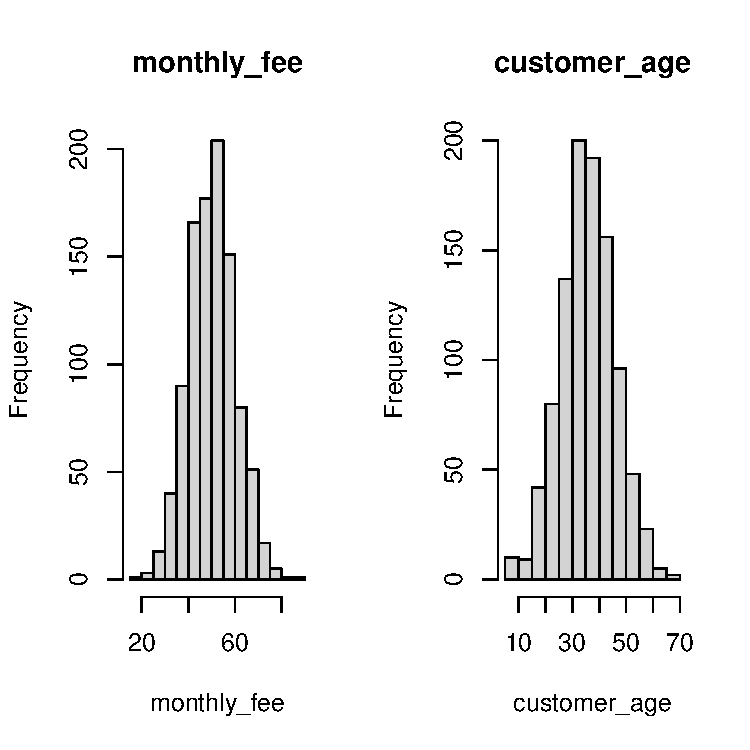
\includegraphics{3_logistic_regression_files/figure-latex/visualization_histogram-1.pdf}
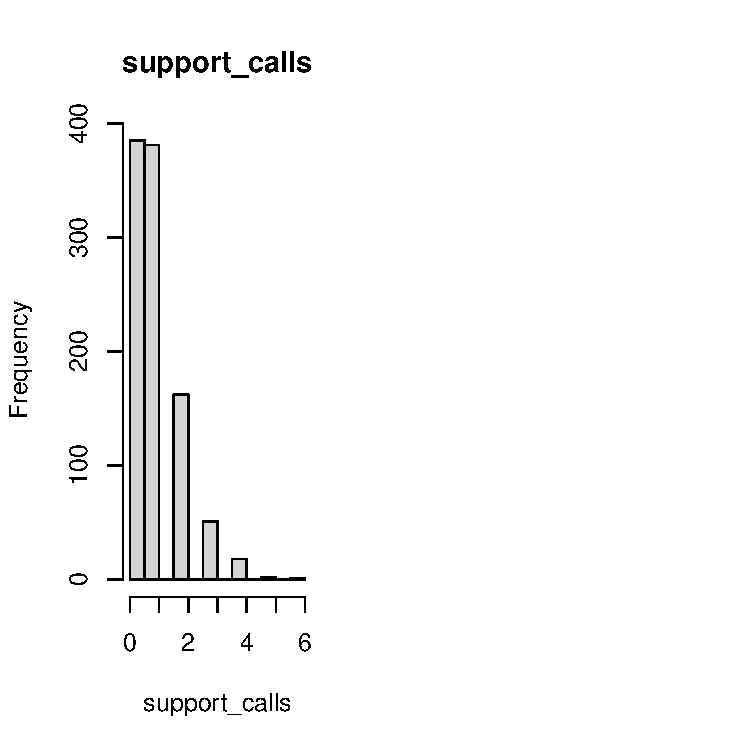
\includegraphics{3_logistic_regression_files/figure-latex/visualization_histogram-2.pdf}

\subsubsection{Box and Whisker Plot}\label{box-and-whisker-plot}

\begin{Shaded}
\begin{Highlighting}[]
\FunctionTok{par}\NormalTok{(}\AttributeTok{mfrow =} \FunctionTok{c}\NormalTok{(}\DecValTok{1}\NormalTok{, }\DecValTok{2}\NormalTok{))}
\ControlFlowTok{for}\NormalTok{ (i }\ControlFlowTok{in} \DecValTok{1}\SpecialCharTok{:}\DecValTok{4}\NormalTok{) \{}
  \ControlFlowTok{if}\NormalTok{ (}\FunctionTok{is.numeric}\NormalTok{(subscription\_churn\_data[[i]])) \{}
    \FunctionTok{boxplot}\NormalTok{(subscription\_churn\_data[[i]], }\AttributeTok{main =} \FunctionTok{names}\NormalTok{(subscription\_churn\_data)[i])}
\NormalTok{  \} }\ControlFlowTok{else}\NormalTok{ \{}
    \FunctionTok{message}\NormalTok{(}\FunctionTok{paste}\NormalTok{(}\StringTok{"Column"}\NormalTok{, }\FunctionTok{names}\NormalTok{(subscription\_churn\_data)[i],}
                  \StringTok{"is not numeric and will be skipped."}\NormalTok{))}
\NormalTok{  \}}
\NormalTok{\}}
\end{Highlighting}
\end{Shaded}

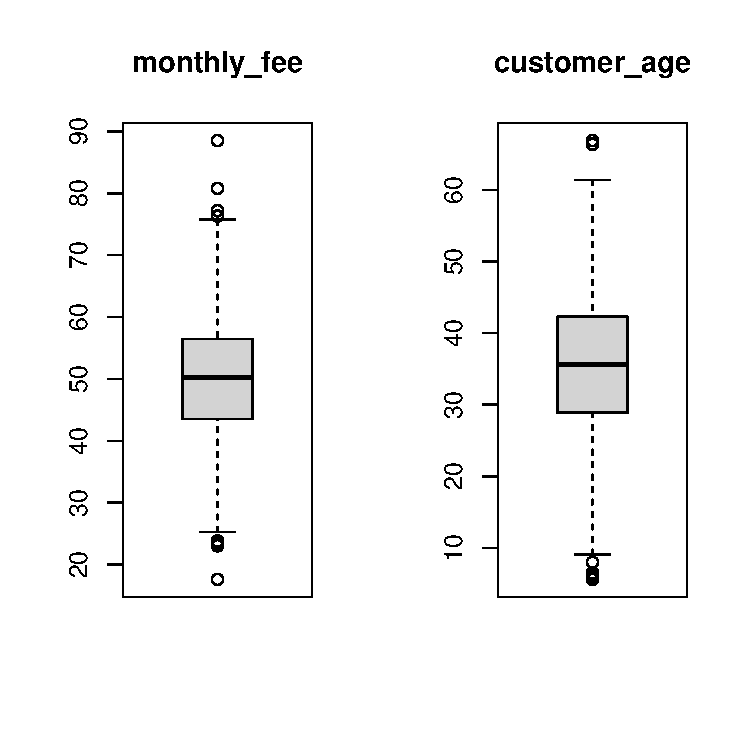
\includegraphics{3_logistic_regression_files/figure-latex/visualization_boxplot-1.pdf}
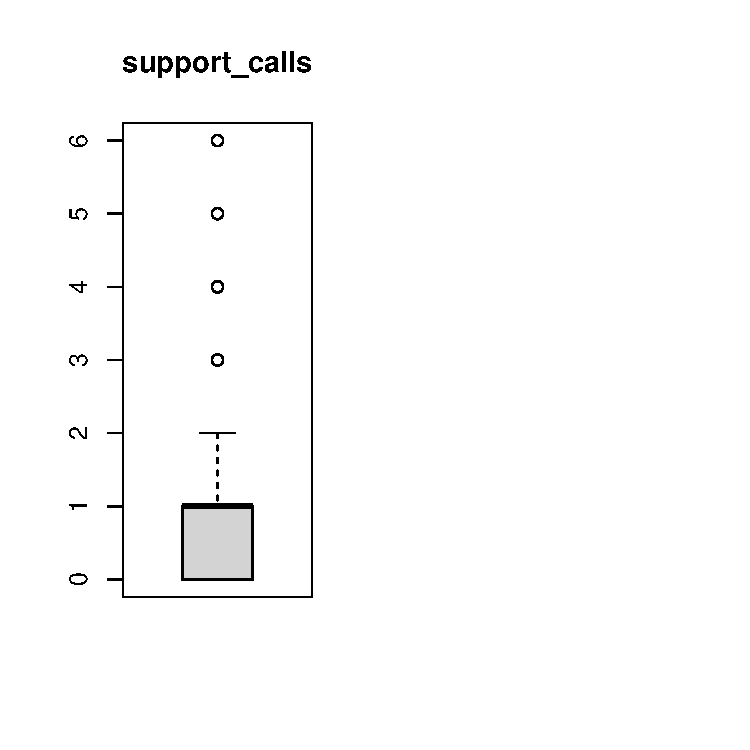
\includegraphics{3_logistic_regression_files/figure-latex/visualization_boxplot-2.pdf}

\subsubsection{Missing Data Plot}\label{missing-data-plot}

\begin{Shaded}
\begin{Highlighting}[]
\NormalTok{pacman}\SpecialCharTok{::}\FunctionTok{p\_load}\NormalTok{(}\StringTok{"Amelia"}\NormalTok{)}

\FunctionTok{missmap}\NormalTok{(subscription\_churn\_data, }\AttributeTok{col =} \FunctionTok{c}\NormalTok{(}\StringTok{"red"}\NormalTok{, }\StringTok{"grey"}\NormalTok{), }\AttributeTok{legend =} \ConstantTok{TRUE}\NormalTok{)}
\end{Highlighting}
\end{Shaded}

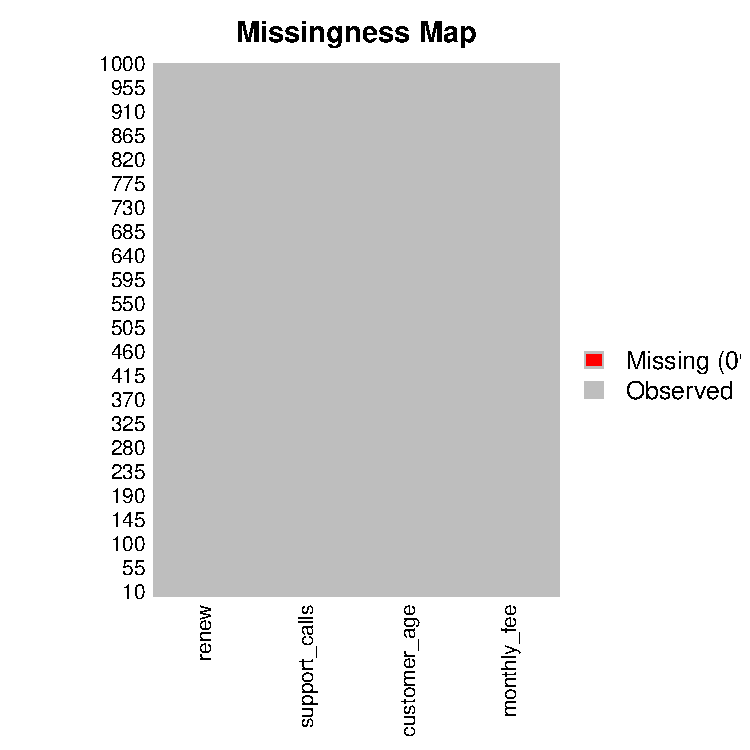
\includegraphics{3_logistic_regression_files/figure-latex/missing_data_plot-1.pdf}

\subsubsection{Correlation Plot}\label{correlation-plot}

\begin{Shaded}
\begin{Highlighting}[]
\NormalTok{pacman}\SpecialCharTok{::}\FunctionTok{p\_load}\NormalTok{(}\StringTok{"ggcorrplot"}\NormalTok{)}

\FunctionTok{ggcorrplot}\NormalTok{(}\FunctionTok{cor}\NormalTok{(subscription\_churn\_data[,}\DecValTok{1}\SpecialCharTok{:}\DecValTok{3}\NormalTok{]))}
\end{Highlighting}
\end{Shaded}

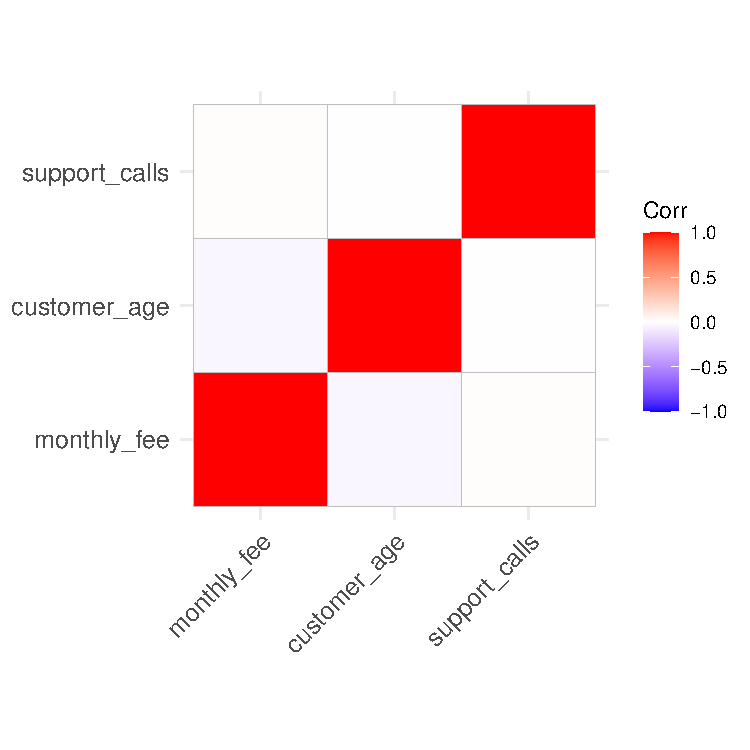
\includegraphics{3_logistic_regression_files/figure-latex/correlation_plot-1.pdf}

\subsubsection{Scatter Plot}\label{scatter-plot}

\begin{Shaded}
\begin{Highlighting}[]
\NormalTok{pacman}\SpecialCharTok{::}\FunctionTok{p\_load}\NormalTok{(}\StringTok{"corrplot"}\NormalTok{)}

\FunctionTok{pairs}\NormalTok{(renew }\SpecialCharTok{\textasciitilde{}}\NormalTok{ ., }\AttributeTok{data =}\NormalTok{ subscription\_churn\_data, }\AttributeTok{col =}\NormalTok{ subscription\_churn\_data}\SpecialCharTok{$}\NormalTok{renew)}
\end{Highlighting}
\end{Shaded}

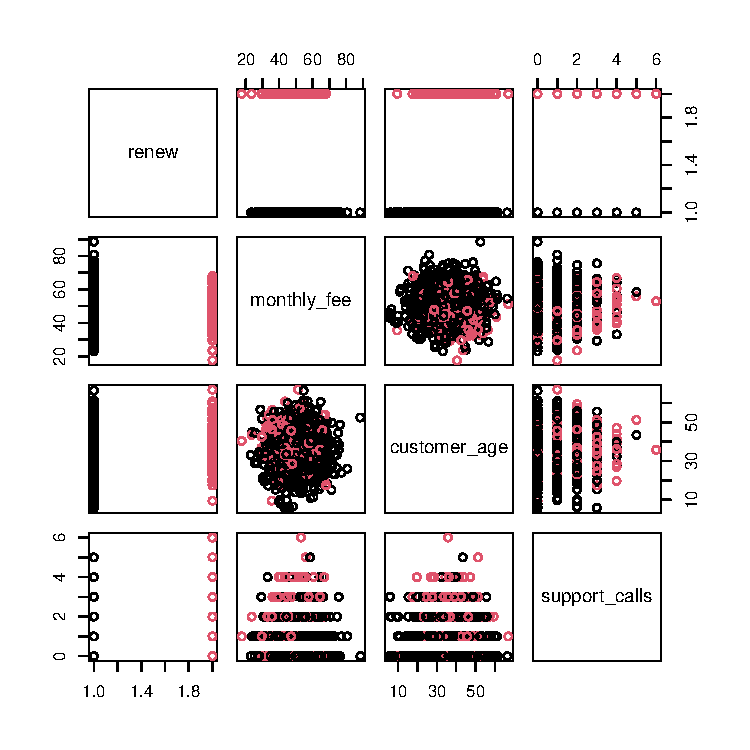
\includegraphics{3_logistic_regression_files/figure-latex/scatter_plot_1-1.pdf}

\begin{Shaded}
\begin{Highlighting}[]
\NormalTok{pacman}\SpecialCharTok{::}\FunctionTok{p\_load}\NormalTok{(}\StringTok{"ggplot2"}\NormalTok{)}
\FunctionTok{ggplot}\NormalTok{(subscription\_churn\_data,}
       \FunctionTok{aes}\NormalTok{(}\AttributeTok{x =}\NormalTok{ customer\_age, }\AttributeTok{y =}\NormalTok{ monthly\_fee)) }\SpecialCharTok{+} 
  \FunctionTok{geom\_point}\NormalTok{() }\SpecialCharTok{+}
  \FunctionTok{geom\_smooth}\NormalTok{(}\AttributeTok{method =}\NormalTok{ lm) }\SpecialCharTok{+}
  \FunctionTok{labs}\NormalTok{(}
    \AttributeTok{title =} \StringTok{"Relationship between Monthly Fee and }\SpecialCharTok{\textbackslash{}n}\StringTok{Customer Age"}\NormalTok{,}
    \AttributeTok{x =} \StringTok{"Customer Age"}\NormalTok{,}
    \AttributeTok{y =} \StringTok{"Monthly Fee"}
\NormalTok{  )}
\end{Highlighting}
\end{Shaded}

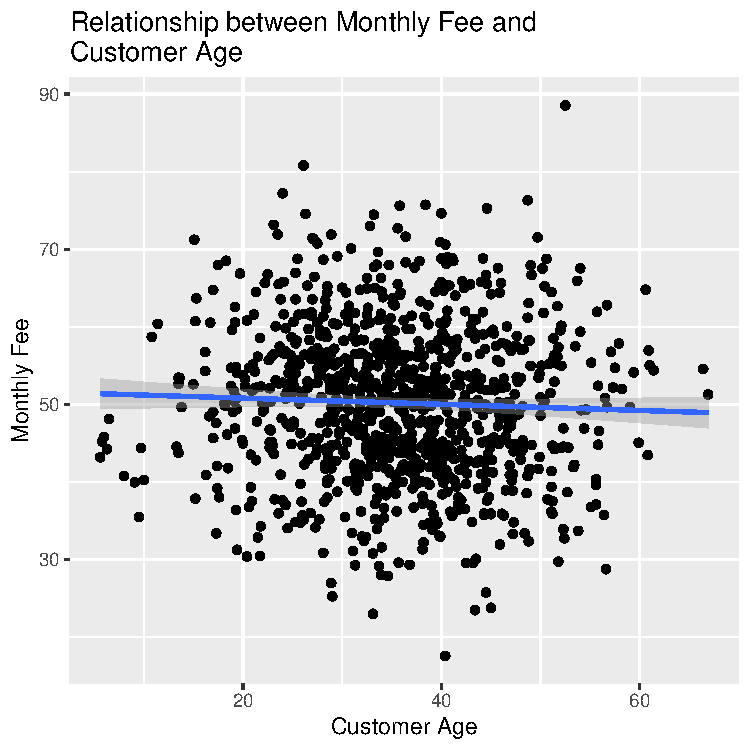
\includegraphics{3_logistic_regression_files/figure-latex/scatter_plot_2-1.pdf}

\begin{Shaded}
\begin{Highlighting}[]
\NormalTok{pacman}\SpecialCharTok{::}\FunctionTok{p\_load}\NormalTok{(}\StringTok{"ggplot2"}\NormalTok{)}
\FunctionTok{ggplot}\NormalTok{(subscription\_churn\_data,}
       \FunctionTok{aes}\NormalTok{(}\AttributeTok{x =}\NormalTok{ customer\_age, }\AttributeTok{y =}\NormalTok{ monthly\_fee, }\AttributeTok{color =}\NormalTok{ renew)) }\SpecialCharTok{+} 
  \FunctionTok{geom\_point}\NormalTok{() }\SpecialCharTok{+}
  \FunctionTok{geom\_smooth}\NormalTok{(}\AttributeTok{method =}\NormalTok{ lm) }\SpecialCharTok{+}
  \FunctionTok{labs}\NormalTok{(}
    \AttributeTok{title =} \StringTok{"Relationship between Monthly Fee and }\SpecialCharTok{\textbackslash{}n}\StringTok{Customer Age for Each Renewal Status"}\NormalTok{,}
    \AttributeTok{x =} \StringTok{"Customer Age"}\NormalTok{,}
    \AttributeTok{y =} \StringTok{"Monthly Fee"}\NormalTok{,}
    \AttributeTok{color =} \StringTok{"Renewal Status"}
\NormalTok{  ) }\SpecialCharTok{+}
  \FunctionTok{scale\_color\_discrete}\NormalTok{(}
    \AttributeTok{labels =} \FunctionTok{c}\NormalTok{(}\StringTok{"1"} \OtherTok{=} \StringTok{"Renewed Subscription"}\NormalTok{, }\StringTok{"0"} \OtherTok{=} \StringTok{"Cancelled Subscription"}\NormalTok{)}
\NormalTok{  ) }\SpecialCharTok{+} 
  \FunctionTok{theme\_minimal}\NormalTok{()  }\CommentTok{\# Optional: adds a cleaner theme}
\end{Highlighting}
\end{Shaded}

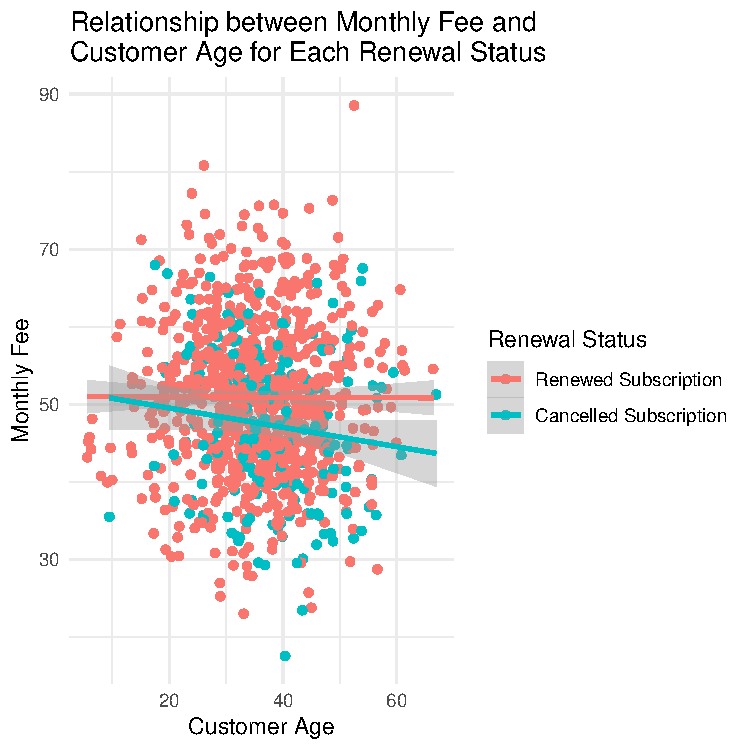
\includegraphics{3_logistic_regression_files/figure-latex/scatter_plot_3-1.pdf}

\section{Statistical Test}\label{statistical-test}

We then apply a logistic regression as a statistical test for
regression.

View the summary of the model.

\begin{Shaded}
\begin{Highlighting}[]
\FunctionTok{summary}\NormalTok{(log\_test)}
\end{Highlighting}
\end{Shaded}

\begin{verbatim}
## 
## Call:
## glm(formula = renew ~ monthly_fee + customer_age + support_calls, 
##     family = binomial, data = subscription_churn_data)
## 
## Coefficients:
##                Estimate Std. Error z value Pr(>|z|)    
## (Intercept)   -0.941778   0.545980  -1.725  0.08454 .  
## monthly_fee   -0.043563   0.008934  -4.876 1.08e-06 ***
## customer_age   0.026110   0.008451   3.089  0.00201 ** 
## support_calls  0.697795   0.081536   8.558  < 2e-16 ***
## ---
## Signif. codes:  0 '***' 0.001 '**' 0.01 '*' 0.05 '.' 0.1 ' ' 1
## 
## (Dispersion parameter for binomial family taken to be 1)
## 
##     Null deviance: 1017.22  on 999  degrees of freedom
## Residual deviance:  906.19  on 996  degrees of freedom
## AIC: 914.19
## 
## Number of Fisher Scoring iterations: 4
\end{verbatim}

The logistic regression equation is in the following form:

\[
\text{log-odds(renew)} = \beta_0 + \beta_1 \cdot fee + \beta_2 \cdot age + \beta_3 \cdot calls
\]

Plugging in the coefficients from the output gives:

\[
\text{log-odds(renew)} = -0.941778 + -0.043563 \cdot fee + 0.026110 \cdot age + 0.697795 \cdot calls
\]

The log-odds is then converted into a probability using the logistic
function as:

\[
P(\text{renew = 1}) = \frac{1}{1+e^{-\text{log-odds}}}
\]

\begin{itemize}
\item
  If P(renew=1)≥0.5, predict renewal of subscription(1).
\item
  If P(renew=1)\textless0.5, predict cancellation of subscription (0).
\end{itemize}

For example, a monthly fee of 50, customer age of 62, and 3 support
calls in the past month is probably going to renew their subscription:

\begin{Shaded}
\begin{Highlighting}[]
\NormalTok{coefs }\OtherTok{\textless{}{-}} \FunctionTok{coef}\NormalTok{(log\_test)}
\NormalTok{log\_odds   }\OtherTok{\textless{}{-}}\NormalTok{ coefs[}\StringTok{"(Intercept)"}\NormalTok{] }\SpecialCharTok{+} 
\NormalTok{  coefs[}\StringTok{"monthly\_fee"}\NormalTok{] }\SpecialCharTok{*} \DecValTok{50} \SpecialCharTok{+}
\NormalTok{  coefs[}\StringTok{"customer\_age"}\NormalTok{] }\SpecialCharTok{*} \DecValTok{62} \SpecialCharTok{+}
\NormalTok{  coefs[}\StringTok{"support\_calls"}\NormalTok{] }\SpecialCharTok{*} \DecValTok{3}

\NormalTok{p\_manual }\OtherTok{\textless{}{-}} \DecValTok{1} \SpecialCharTok{/}\NormalTok{ (}\DecValTok{1} \SpecialCharTok{+} \FunctionTok{exp}\NormalTok{(}\SpecialCharTok{{-}}\NormalTok{log\_odds))}

\FunctionTok{print}\NormalTok{(p\_manual)}
\end{Highlighting}
\end{Shaded}

\begin{verbatim}
## (Intercept) 
##   0.6438873
\end{verbatim}

For example, a monthly fee of 50, customer age of 21, and 3 support
calls in the past month is probably going to cancel their subscription:

\begin{Shaded}
\begin{Highlighting}[]
\NormalTok{coefs }\OtherTok{\textless{}{-}} \FunctionTok{coef}\NormalTok{(log\_test)}
\NormalTok{log\_odds   }\OtherTok{\textless{}{-}}\NormalTok{ coefs[}\StringTok{"(Intercept)"}\NormalTok{] }\SpecialCharTok{+} 
\NormalTok{  coefs[}\StringTok{"monthly\_fee"}\NormalTok{] }\SpecialCharTok{*} \DecValTok{50} \SpecialCharTok{+}
\NormalTok{  coefs[}\StringTok{"customer\_age"}\NormalTok{] }\SpecialCharTok{*} \DecValTok{21} \SpecialCharTok{+}
\NormalTok{  coefs[}\StringTok{"support\_calls"}\NormalTok{] }\SpecialCharTok{*} \DecValTok{3}

\NormalTok{p\_manual }\OtherTok{\textless{}{-}} \DecValTok{1} \SpecialCharTok{/}\NormalTok{ (}\DecValTok{1} \SpecialCharTok{+} \FunctionTok{exp}\NormalTok{(}\SpecialCharTok{{-}}\NormalTok{log\_odds))}

\FunctionTok{print}\NormalTok{(p\_manual)}
\end{Highlighting}
\end{Shaded}

\begin{verbatim}
## (Intercept) 
##    0.382672
\end{verbatim}

\subsection{\texorpdfstring{The \(\chi^2\) Statistic and its
p-Value}{The \textbackslash chi\^{}2 Statistic and its p-Value}}\label{the-chi2-statistic-and-its-p-value}

To obtain the p-value of the \(\chi^2\) statistic:

\begin{Shaded}
\begin{Highlighting}[]
\CommentTok{\# chi\_2 \textless{}{-} log\_test$null.deviance/1 {-} log\_test$residuals}
\NormalTok{chi\_2 }\OtherTok{\textless{}{-}} \FloatTok{1017.22} \SpecialCharTok{{-}} \FloatTok{906.19}

\FunctionTok{print}\NormalTok{(chi\_2)}
\end{Highlighting}
\end{Shaded}

\begin{verbatim}
## [1] 111.03
\end{verbatim}

\begin{Shaded}
\begin{Highlighting}[]
\NormalTok{p }\OtherTok{\textless{}{-}} \DecValTok{1} \SpecialCharTok{{-}} \FunctionTok{pchisq}\NormalTok{(chi\_2, }\AttributeTok{df =} \DecValTok{3}\NormalTok{)}
\CommentTok{\# to format as a scientific notation with four digits after the decimal place}
\CommentTok{\# sprintf("\%.4e", p)}
\FunctionTok{format.pval}\NormalTok{(p, }\AttributeTok{eps =}\NormalTok{ .Machine}\SpecialCharTok{$}\NormalTok{double.eps, }\AttributeTok{digits =} \DecValTok{2}\NormalTok{)}
\end{Highlighting}
\end{Shaded}

\begin{verbatim}
## [1] "<2e-16"
\end{verbatim}

\subsection{95\% Confidence Interval of the
Parameters}\label{confidence-interval-of-the-parameters}

To obtain a 95\% confidence interval for the parameters:

\begin{Shaded}
\begin{Highlighting}[]
\FunctionTok{confint}\NormalTok{(log\_test, }\AttributeTok{level =} \FloatTok{0.95}\NormalTok{)}
\end{Highlighting}
\end{Shaded}

\begin{verbatim}
##                      2.5 %      97.5 %
## (Intercept)   -2.018238039  0.12436807
## monthly_fee   -0.061306856 -0.02624538
## customer_age   0.009645052  0.04281132
## support_calls  0.540327294  0.86041171
\end{verbatim}

\subsection{Odds Ratio}\label{odds-ratio}

Exponentiating the coefficients yields odds ratios, which quantify the
multiplicative change in odds for a one‑unit increase in the predictor.

\begin{Shaded}
\begin{Highlighting}[]
\FunctionTok{exp}\NormalTok{(}\FunctionTok{coef}\NormalTok{(log\_test))}
\end{Highlighting}
\end{Shaded}

\begin{verbatim}
##   (Intercept)   monthly_fee  customer_age support_calls 
##     0.3899341     0.9573725     1.0264536     2.0093179
\end{verbatim}

\subsubsection{95\% Confidence Interval for the Odds
Ratio}\label{confidence-interval-for-the-odds-ratio}

To obtain a 95\% confidence interval for the Odds Ratio:

\begin{Shaded}
\begin{Highlighting}[]
\NormalTok{pacman}\SpecialCharTok{::}\FunctionTok{p\_load}\NormalTok{(}\StringTok{"dplyr"}\NormalTok{)}
\FunctionTok{confint}\NormalTok{(log\_test) }\SpecialCharTok{\%\textgreater{}\%} \FunctionTok{exp}\NormalTok{()}
\end{Highlighting}
\end{Shaded}

\begin{verbatim}
##                   2.5 %   97.5 %
## (Intercept)   0.1328894 1.132433
## monthly_fee   0.9405346 0.974096
## customer_age  1.0096917 1.043741
## support_calls 1.7165686 2.364134
\end{verbatim}

\subsection{Akaike Information Criterion
(AIC)}\label{akaike-information-criterion-aic}

AIC specifies how well a model fits the data from which it was
generated. The AIC value is calculated using the number of predictor
variables and also the estimate of the maximum likelihood of the model.
AIC penalizes complexity, therefore, any model with a lesser AIC value
is a more significant model. A lower AIC value means the complexity of
the model is lower and the model better explains the variations. The
model's AIC value of 914.19 can be compared with the AIC value of
alternative models, e.g., a logistic regression that has dropped one of
the original predictors.

\subsection{\texorpdfstring{McFadden's Pseudo
R\textsuperscript{2}}{McFadden's Pseudo R2}}\label{mcfaddens-pseudo-r2}

Logistic regression does not use the traditional R², but we can compute
a \textbf{pseudo-R²} (McFadden's) as follows:

\begin{Shaded}
\begin{Highlighting}[]
\NormalTok{pseudo\_r2 }\OtherTok{\textless{}{-}} \DecValTok{1} \SpecialCharTok{{-}}\NormalTok{ (log\_test}\SpecialCharTok{$}\NormalTok{deviance }\SpecialCharTok{/}\NormalTok{ log\_test}\SpecialCharTok{$}\NormalTok{null.deviance)}
\FunctionTok{print}\NormalTok{(pseudo\_r2)}
\end{Highlighting}
\end{Shaded}

\begin{verbatim}
## [1] 0.1091487
\end{verbatim}

A McFadden's pseudo-R\textsuperscript{2} of 0.109 suggests that the
predictors explain approximately 10.91\% of the variance in the outcome.
pseudo-R\textsuperscript{2} \textgreater{} 0.2 are considered strong in
logistic regression.

\subsection{Fisher Scoring Iterations}\label{fisher-scoring-iterations}

There were 4 Fisher scoring iterations which indicates that the fitting
routine required four iterative updates to reach convergence. A small
number (\textless{} 10) suggests that the algorithm found the
maximum-likelihood estimates efficiently without convergence warnings.

\subsection{Model Fit Metrics}\label{model-fit-metrics}

The ROC Curve and the AUC gives insight into how well the logistic
regression model distinguishes between the two outcome classes (1 =
renew and 0 = cancel).

\begin{itemize}
\item
  The x-axis shows the False Positive Rate (FPR), or specificity.
\item
  The y-axis shows the True Positive Rate (TPR), or sensitivity.
\item
  The curve shows how TPR and FPR change as the decision threshold
  changes from 0 to 1.
\item
  A curve closer to the top-left corner indicates better model
  performance.
\end{itemize}

\begin{Shaded}
\begin{Highlighting}[]
\NormalTok{pacman}\SpecialCharTok{::}\FunctionTok{p\_load}\NormalTok{(}\StringTok{"pROC"}\NormalTok{)}

\NormalTok{predicted\_probs }\OtherTok{\textless{}{-}} \FunctionTok{predict}\NormalTok{(log\_test, }\AttributeTok{type =} \StringTok{"response"}\NormalTok{)}

\NormalTok{roc\_obj }\OtherTok{\textless{}{-}} \FunctionTok{roc}\NormalTok{(subscription\_churn\_data}\SpecialCharTok{$}\NormalTok{renew, predicted\_probs)}
\NormalTok{auc\_value }\OtherTok{\textless{}{-}} \FunctionTok{auc}\NormalTok{(roc\_obj)}
\FunctionTok{plot}\NormalTok{(roc\_obj, }\AttributeTok{col =} \StringTok{"blue"}\NormalTok{, }\AttributeTok{main =} \StringTok{"ROC Curve for Logistic Regression"}\NormalTok{)}
\end{Highlighting}
\end{Shaded}

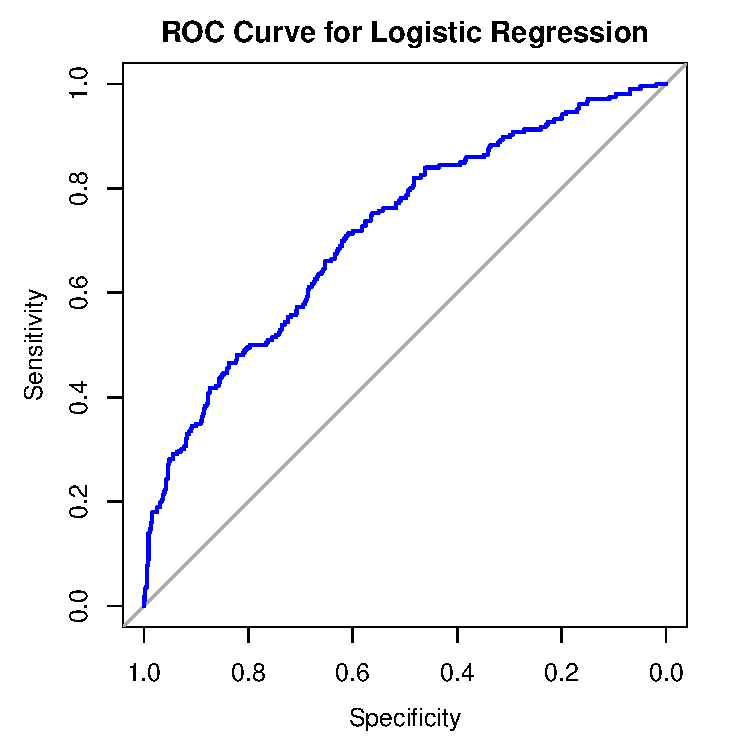
\includegraphics{3_logistic_regression_files/figure-latex/model_fit_a-1.pdf}

\begin{Shaded}
\begin{Highlighting}[]
\FunctionTok{print}\NormalTok{(auc\_value)}
\end{Highlighting}
\end{Shaded}

\begin{verbatim}
## Area under the curve: 0.7167
\end{verbatim}

\begin{longtable}[]{@{}
  >{\raggedright\arraybackslash}p{(\columnwidth - 2\tabcolsep) * \real{0.5000}}
  >{\raggedright\arraybackslash}p{(\columnwidth - 2\tabcolsep) * \real{0.5000}}@{}}
\caption{AUC Value Interpretation}\tabularnewline
\toprule\noalign{}
\begin{minipage}[b]{\linewidth}\raggedright
AUC Value
\end{minipage} & \begin{minipage}[b]{\linewidth}\raggedright
Interpretation
\end{minipage} \\
\midrule\noalign{}
\endfirsthead
\toprule\noalign{}
\begin{minipage}[b]{\linewidth}\raggedright
AUC Value
\end{minipage} & \begin{minipage}[b]{\linewidth}\raggedright
Interpretation
\end{minipage} \\
\midrule\noalign{}
\endhead
\bottomrule\noalign{}
\endlastfoot
0.5 & Using the logistic regression model is equivalent to randomly
guessing \\
0.6 - 0.7 & Poor discrimination of the classes \\
0.7 - 0.8 & Acceptable discrimination of the classes (fair) \\
0.8 - 0.9 & Good discrimination \\
0.9 - 1.0 & Excellent discrimination \\
\end{longtable}

An AUC of 0.7167 indicates that the model has an acceptable ability to
discriminate between the two classes.

\section{Diagnostic EDA}\label{diagnostic-eda}

Diagnostic EDA is performed to validate that the regression assumptions
are true with respect to the statistical test. Validating the regression
assumption in turn ensures that the statistical tests applied are
appropriate for the data and helps to prevent incorrect conclusions.

\subsection{Test of Linearity}\label{test-of-linearity}

The test of linearity is necessary given that linearity is one of the
key assumptions of statistical tests of regression and verifying it is
crucial for ensuring the validity of the model's estimates and
predictions.

\textbf{Component-Plus-Residual (Partial-Residual) Plots}

Logistic regression assumes that the relationship between the logit
(log-odds) of the outcome and the continuous predictors is linear. A
logit is the natural logarithm of the odds of an event occurring, i.e.,
if \emph{p} is the probability of an event (where 0 \textless{} \emph{p}
\textless{} 1), the odds are \(\frac{p}{1 - p}\) and the logit is:

\[ \text{logit}(p) = \ln\left(\frac{p}{1-p}\right) \]

A roughly straight line indicates the logit-predictor linearity
assumption is met.

\begin{Shaded}
\begin{Highlighting}[]
\NormalTok{pacman}\SpecialCharTok{::}\FunctionTok{p\_load}\NormalTok{(}\StringTok{"car"}\NormalTok{)}

\FunctionTok{crPlots}\NormalTok{(log\_test)}
\end{Highlighting}
\end{Shaded}

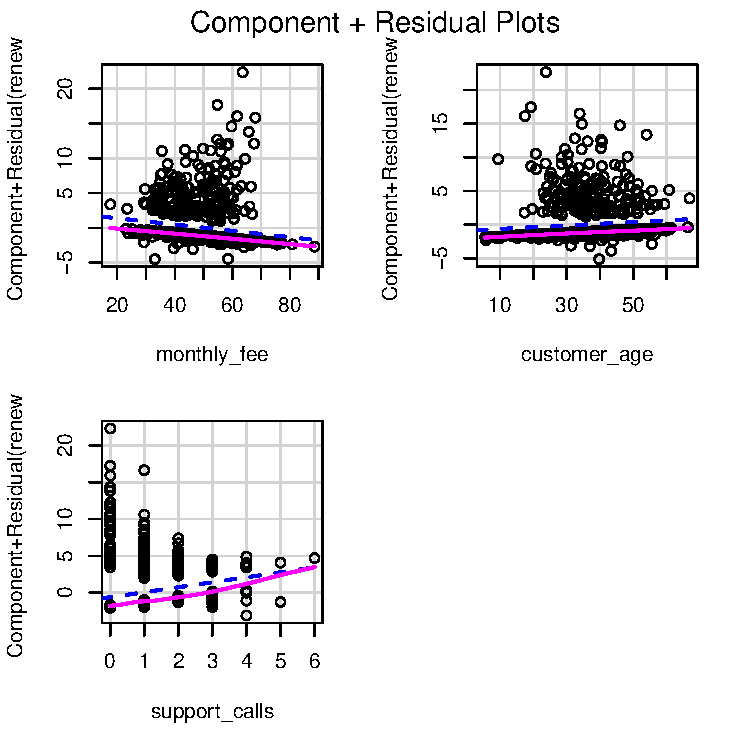
\includegraphics{3_logistic_regression_files/figure-latex/test_of_linearity-1.pdf}

\subsection{Test of Independence of
Errors}\label{test-of-independence-of-errors}

This test is necessary to confirm that each observation is independent
of the other. It helps to identify \textbf{autocorrelation} that is
introduced when the data is collected over a close period of time or
when one observation is related to another observation. Autocorrelation
leads to underestimated standard errors and inflated t-statistics. It
can also make findings appear more significant than they actually are.

The ``\textbf{Durbin-Watson Test}'' can be used as a test of
independence of errors (test of autocorrelation).

\begin{itemize}
\item
  The null hypothesis, H\textsubscript{0}, is that there is no
  autocorrelation
\item
  The alternative hypothesis, H\textsubscript{a}, is that there is
  autocorrelation
\end{itemize}

If the p-value is greater than 0.05 then there is no evidence to reject
the null hypothesis that ``there is no autocorrelation''. The results
below show \emph{p} \textgreater{} 0.05, therefore, the test of
independence of errors around the regression line passes.

\begin{Shaded}
\begin{Highlighting}[]
\NormalTok{pacman}\SpecialCharTok{::}\FunctionTok{p\_load}\NormalTok{(}\StringTok{"lmtest"}\NormalTok{)}
\FunctionTok{dwtest}\NormalTok{(log\_test)}
\end{Highlighting}
\end{Shaded}

\begin{verbatim}
## 
##  Durbin-Watson test
## 
## data:  log_test
## DW = 2.0912, p-value = 0.9258
## alternative hypothesis: true autocorrelation is greater than 0
\end{verbatim}

\subsection{Test of Normality}\label{test-of-normality}

Logistic regression does not assume normality of residuals or
predictors.

\subsection{Test of Homoscedasticity}\label{test-of-homoscedasticity}

The test of homoscedasticity is not relevant for logistic regression.

\subsection{Test of Multicollinearity}\label{test-of-multicollinearity}

Multicollinearity arises when two or more independent variables
(predictors) are highly intercorrelated. The \textbf{Variance Inflation
Factor (VIF)} quantifies how much the variance of a coefficient estimate
is ``inflated'' due to multicollinearity. A VIF of 1 indicates no
collinearity; values above 5 suggest problematic levels of collinearity.
High VIF values (VIF \textgreater{} 5) suggest that the coefficient
estimates are less reliable due to the correlations between predictors.

\begin{Shaded}
\begin{Highlighting}[]
\NormalTok{pacman}\SpecialCharTok{::}\FunctionTok{p\_load}\NormalTok{(}\StringTok{"car"}\NormalTok{)}
\FunctionTok{vif}\NormalTok{(log\_test)}
\end{Highlighting}
\end{Shaded}

\begin{verbatim}
##   monthly_fee  customer_age support_calls 
##      1.017865      1.003913      1.020388
\end{verbatim}

\subsection{Test of Outliers}\label{test-of-outliers}

The \texttt{influencePlot()} function in R combines 3 key diagnostic
measures into a single plot to identify influential observations.

The plot displays:

\begin{itemize}
\item
  Y-axis: Studentized residuals (standardized residuals adjusted for
  leverage).
\item
  X-axis: Leverage (hat values), measuring how ``unusual'' an
  observation is in terms of its predictor values.
\item
  Bubble size: Cook's distance, quantifying the influence of each
  observation on the model coefficients.
\end{itemize}

Top-left/bottom-left:

\begin{itemize}
\item
  Indicates observations with high residuals but low leverage: Outliers
  in the outcome but not predictors.
\item
  Possible next step: Investigate the observations for misclassified
  outcomes.
\end{itemize}

Top-right/bottom-right:

\begin{itemize}
\item
  Indicates high residuals and high leverage: Influential outliers that
  distort the model.
\item
  Possible next step: These are the most problematic observations. You
  need to check if they are valid data points or errors.
\end{itemize}

Middle-right:

\begin{itemize}
\item
  High leverage but residuals near 0: Unusual predictor values but
  well-predicted outcomes.
\item
  Possible next step: These observations are generally safe to keep.
\end{itemize}

\begin{Shaded}
\begin{Highlighting}[]
\NormalTok{pacman}\SpecialCharTok{::}\FunctionTok{p\_load}\NormalTok{(}\StringTok{"car"}\NormalTok{)}

\FunctionTok{influencePlot}\NormalTok{(log\_test, }
              \AttributeTok{id =} \FunctionTok{list}\NormalTok{(}\AttributeTok{n =} \DecValTok{5}\NormalTok{),  }\CommentTok{\# Label top 5 influential points}
              \AttributeTok{main =} \StringTok{"Influence Plot"}\NormalTok{,}
              \AttributeTok{sub =} \StringTok{"Circle size = Cook\textquotesingle{}s Distance"}\NormalTok{)}
\end{Highlighting}
\end{Shaded}

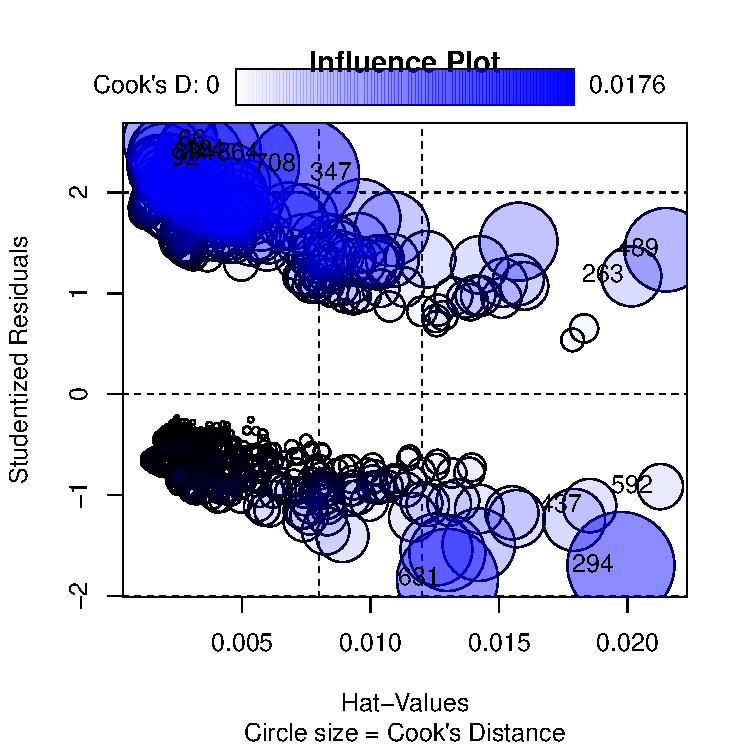
\includegraphics{3_logistic_regression_files/figure-latex/outliers_plot-1.pdf}

\begin{verbatim}
##        StudRes         Hat       CookD
## 66   2.5131733 0.002206220 0.012165628
## 92   2.3329288 0.001942625 0.006822822
## 184  2.4100283 0.002433914 0.010319622
## 263  1.1669909 0.020141623 0.005015865
## 294 -1.6986014 0.019738247 0.015927999
## 347  2.1803805 0.007365365 0.017572966
## 437 -1.1050303 0.018518805 0.003975203
## 489  1.4311225 0.021496490 0.009721397
## 592 -0.9163872 0.021272184 0.002849801
## 631 -1.8366802 0.012990570 0.014176667
## 708  2.2742892 0.005166374 0.015498587
## 864  2.3828386 0.003736612 0.014686885
## 894  2.3758317 0.002043544 0.007976687
\end{verbatim}

The influential outliers can then be:

\begin{enumerate}
\def\labelenumi{\arabic{enumi}.}
\item
  Corrected for data entry errors, e.g., an age of 240 years
\item
  Deleted so that the statistical test can be run again without them
\end{enumerate}

Print the observation numbers that have been identified as influential
outliers

\begin{Shaded}
\begin{Highlighting}[]
\FunctionTok{print}\NormalTok{(influential\_points)}
\end{Highlighting}
\end{Shaded}

\begin{verbatim}
## [1]  66 184 294 347 489 592
\end{verbatim}

Print the influential observations' predictor and outcome values.

\begin{Shaded}
\begin{Highlighting}[]
\FunctionTok{head}\NormalTok{(subscription\_churn\_data\_infl)}
\end{Highlighting}
\end{Shaded}

\begin{verbatim}
## # A tibble: 6 x 4
##   monthly_fee customer_age support_calls renew
##         <dbl>        <dbl>         <int> <fct>
## 1        63.6         23.8             0 0    
## 2        54.8         19.3             0 0    
## 3        58.5         43.4             5 1    
## 4        35.5          9.5             0 0    
## 5        66.9         19.7             4 0    
## 6        45.2          5.8             3 1
\end{verbatim}

\section{Interpretation of the
Results}\label{interpretation-of-the-results}

\subsection{Academic Statement}\label{academic-statement}

A logistic regression analysis was conducted on data (N = 1,000) to
examine whether monthly subscription fee paid by a customer, the
customer's age, and the number of support calls the customer made in the
last month predicted the subscription renewal, where renew was coded 1
for subscription renewal and 0 for subscription cancellation.

Subtracting the residual deviance (906.19 on 996 df) from the null
deviance (1,017.22 on 999 df) gave a \(\chi^2\)(3, N = 1,000) = 111.03,
\emph{p} \textless{} .001, thus showing that the model was statistically
significant compared to the null model. The set of predictors reliably
distinguished between renewals and cancellations.

The results are reported in the table below:

\begin{longtable}[]{@{}
  >{\centering\arraybackslash}p{(\columnwidth - 10\tabcolsep) * \real{0.3472}}
  >{\centering\arraybackslash}p{(\columnwidth - 10\tabcolsep) * \real{0.1250}}
  >{\centering\arraybackslash}p{(\columnwidth - 10\tabcolsep) * \real{0.2222}}
  >{\centering\arraybackslash}p{(\columnwidth - 10\tabcolsep) * \real{0.0833}}
  >{\centering\arraybackslash}p{(\columnwidth - 10\tabcolsep) * \real{0.0972}}
  >{\centering\arraybackslash}p{(\columnwidth - 10\tabcolsep) * \real{0.1250}}@{}}
\caption{Regression Coefficients Predicting Renewal from Multiple
Customer Features}\tabularnewline
\toprule\noalign{}
\begin{minipage}[b]{\linewidth}\centering
Predictor
\end{minipage} & \begin{minipage}[b]{\linewidth}\centering
\(\beta\)
\end{minipage} & \begin{minipage}[b]{\linewidth}\centering
95\% CI
\end{minipage} & \begin{minipage}[b]{\linewidth}\centering
SE
\end{minipage} & \begin{minipage}[b]{\linewidth}\centering
\emph{z}
\end{minipage} & \begin{minipage}[b]{\linewidth}\centering
\emph{p}
\end{minipage} \\
\midrule\noalign{}
\endfirsthead
\toprule\noalign{}
\begin{minipage}[b]{\linewidth}\centering
Predictor
\end{minipage} & \begin{minipage}[b]{\linewidth}\centering
\(\beta\)
\end{minipage} & \begin{minipage}[b]{\linewidth}\centering
95\% CI
\end{minipage} & \begin{minipage}[b]{\linewidth}\centering
SE
\end{minipage} & \begin{minipage}[b]{\linewidth}\centering
\emph{z}
\end{minipage} & \begin{minipage}[b]{\linewidth}\centering
\emph{p}
\end{minipage} \\
\midrule\noalign{}
\endhead
\bottomrule\noalign{}
\endlastfoot
(Intercept) & -0.94 & {[}-2.02, 0.12{]} & 0.55 & -1.73 & 0.085 \\
Monthly Fee & -0.04 & {[}-0.06, -0.03{]} & 0.01 & -4.88 & \textless{}
.001 \\
Customer's Age & 0.03 & {[}0.01, 0.04{]} & 0.01 & 3.09 & .002 \\
Number of Support Calls & 0.70 & {[}0.54, 0.86{]} & 0.08 & 8.56 &
\textless{} .001 \\
\end{longtable}

\textbf{\emph{Note.}} N\,=\,1,000; SE\,=\,standard error;
CI\,=\,confidence interval.

\textbf{Predictor Effects}

\begin{itemize}
\item
  The monthly fee (\(\beta\) = -0.04, 95\% CI {[}-0.06, -0.03{]}, SE =
  0.01, \emph{z} = -4.88, \emph{p} \textless{} .001) was the first
  predictor. For every unit increase in monthly fees, the odds of
  renewal decrease by 4\% (\emph{OR} = 0.96, 95\% CI {[}0.94, 0.97{]},
  p\textless{} .001).
\item
  The customer age (\(\beta\) = 0.03, 95\% CI {[}0.01, 0.04{]}, SE =
  0.01, \emph{z} = 3.09, \emph{p} = .002). For every unit increase in
  the customer's age, the odds of renewal increased by 3\% (\emph{OR} =
  1.03, 95\% CI {[}1.01, 1.04{]}, \emph{p} = .002).
\item
  The number of support calls (\(\beta\) = 0.70, 95\% CI {[}0.54,
  0.86{]}, SE = 0.08, \emph{z} = 8.56, \emph{p} \textless{} .001). For
  every unit increase in the number of support calls, the odds of
  renewal increased by 101\% (\emph{OR} = 2.01, 95\% CI {[}1.72,
  2.36{]}, \emph{p} \textless{} .001)
\item
  The intercept term was not statistically significant (\(\beta\) =
  -0.94, 95 \% CI {[}-2.02, 0.12{]}, SE = 0.55, \emph{z} = -1.73,
  \emph{p} = 0.085) thus indicating no significant baseline odds of
  renewal when all predictors are zero.
\end{itemize}

\subsection{Business Analysis}\label{business-analysis}

Key insights:

\begin{enumerate}
\def\labelenumi{\arabic{enumi}.}
\item
  Monthly Fee:

  \begin{itemize}
  \item
    Finding: Higher monthly fees significantly reduce renewal odds (−4\%
    per unit increase in monthly fee).
  \item
    Implication: Customers are price-sensitive; fee hikes risk
    cancellations.
  \item
    Recommendation: Avoid aggressive fee increases. Consider small,
    incremental fee adjustments for high-value customers.
  \end{itemize}
\item
  Customer Age:

  \begin{itemize}
  \item
    Finding: Older customers are more likely to renew (+3\% odds per
    year of age).
  \item
    Implication: Younger customers may need targeted retention efforts.
  \item
    Recommendation: Launch engagement campaigns, e.g., personalized
    offers
  \end{itemize}
\item
  Support Calls:

  \begin{itemize}
  \item
    Finding: Each support call doubles renewal odds (+101\% per unit
    increase in support calls).
  \item
    Implication: Proactive customer support drives loyalty and
    retention.
  \item
    Recommendations:

    \begin{itemize}
    \item
      Train customer care officers to resolve issues fully and to
      anticipate needs, e.g., follow-up calls after ticket closure
    \item
      Avoid over-reliance on support calls: High call volumes may
      indicate unresolved product issues.
    \end{itemize}
  \end{itemize}
\end{enumerate}

\subsection{Limitations}\label{limitations}

\begin{enumerate}
\def\labelenumi{\arabic{enumi}.}
\item
  Logistic regression performs poorly with small datasets or rare events
  (e.g., very few cancellations). Renewal rates are imbalanced, 79.4\%
  renewals, therefore, the coefficient estimates could be biased.
\item
  Assumes no clustering (e.g., multiple subscriptions per customer) or
  autocorrelation (e.g., time-series trends).
\item
  Stakeholders may struggle to interpret deviance or AIC values.
\item
  Support Call Paradox: While \texttt{support\_calls} had a strong
  positive effect, excessive calls could signal dissatisfaction (which
  is not captured by the model).
\end{enumerate}

\end{document}
